\section{Validation}


\subsection{Strategies}
We can emulate a variety of toolpath generation strategies by applying various beading strategies to our framework.

\paragraph{Naive Strategy}


\paragraph{Constant bead count}
Emulates \cite{Ding2016a}


\paragraph{Deviation at middle}
Emulates \cite{Jin2017}


\paragraph{Only outer bead}
Emulates \cite{Moesen2011}


\paragraph{Distributed strategy}
Distribute the overfill or underfill which would happen using a naive strategy over all beads.
This maximizes robustness and minimizes narrow beads qhich are difficult to print.


\paragraph{Combined strategy}
\Cref{wedge_and_infill} shows a combined toolpath strategy.

\begin{figure}
\centering
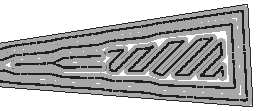
\includegraphics[width=.99\columnwidth]{sources/method/wedge_and_infill.pdf}
\caption{Use single and double wall lines in regions where the infill would be too thin.}
\label{wedge_and_infill}
\end{figure}


\subsection{Filling accuracy}
Render toolpaths and calculate percentage of covered volume.

Visualize thickness of beads as color.

Show results for different settings.

Also render with nozzle size as minimal width and use middle of toolpaths instead of middle of beads.

Take same examples as Moessen: grids of triangular holes and circular holes.
Also use examples of Jin and Kao.

Use example layers of a typical object with thin walls: electronics casing.


